\section{Графы}

Этот параграф не содержит каких-то очень важных для нашего курса сведений — он просто призван служить демонстрацией отдельных понятий, которые мы вводили. Всё, о чем мы говорили до сих пор, может показаться слишком абстрактным и не практичным на первый взгляд, и в этом параграфе я на примере двух задач, очень простой и очень сложной, а так же нестрогих геометрических ассоциаций, покажу, что на самом деле даже то, что я изложил до сих пор, может оказаться вполне полезным, если грамотно это применить. Материал, связанный со второй задачей и многомерной геометрией на самом деле очень жесткий (и одновременно с тем неформальный), так что при первом знакомстве его можно пропустить. (Я вообще не уверен, был ли я прав, это написав).

Если говорить неформально, то граф — это набор точек, называемых вершинами, некоторые из которых соединенны линиями, называемыми рёбрами. Графы бывают многих разновидностей, но нас пока будут интересовать простые графы и ориентированные графы (кратко орграфы), у которых каждое ребро записывается в виде стрелки и называется дугой.

Мы уже встречали графы в прошлом параграфе: диаграммы частично упорядоченных множеств как раз представляют собой орграфы. Графы и орграфы часто используются для описания многих предметов нашей жизни: карта дорог между городами является графом, где дороги — это ребра графа, а города — вершины. Графом является схема компьютерной сети: каждый компьютер в таком графе является вершиной, а кабель, соединяющий их в сеть, является ребром. Ориентированные графы применяются всякими там менеджерами для планирования всяких там задач: у них вершинами графов являются задачи, которые необходимо исполнить, а дугами показывается зависимость между задачами (если из задачи $A$ в задачу $B$ идет стрелочка, то выполнение задачи $B$ не может быть начато до окончания задачи $A$). Инженеры используют разновидности графов для представления электрических цепей. И так далее. Некоторые из этих задач мы будем рассматривать в дальнейшем (в основном в виде простых самостоятельных упражнений).

Важно ответить, что граф — это именно набор вершин и ребер, но не их представление на бумаге. Если изменить форму ребер или положение вершин, граф от этого не изменится, хотя визуально может выглядеть и сильно по-другому. Например, следующие три графа одинаковы (научно говорят изоморфны):

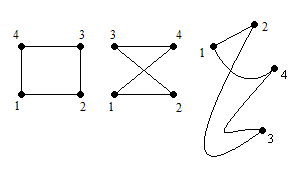
\includegraphics{isomorphic_graphs.png}

Что такое граф интуитивно, думаю, понятно. Давайте теперь все формализуем и определим графы через теорию множеств.

{\bfseries Определение.} {\slshape Графом} называется упорядоченная пара $(V, E)$, где $V$ — множество, элементы которого называются вершинами графа, а $E$ — симметричное антирефлексивное отношение на $V$, элементы которого называются ребрами графа.

{\bfseries Определение.} Если ослабить условия прошлого определения и разрешить, чтобы отношение $E$ не было симметричным, то такая конструкция будет называться {\slshape ориентированным графом}. Сами элементы множества $E$ называются в этом случае {\slshape дугами}.

Мы будем говорить преимущественно о неориентируемых графах. В общем случае антирефлексивность не требуется, но мы для простоты будем исключать из рассмотрения ребра вида $(a, a)$, чтобы не отвлекаться на различные частные случаи.

{\bfseries Определение.} Если $(v, w) \in E$, то вершины $v$ и $w$ называются {\slshape инцидентными}. Так же говорят, что $v$ и $w$ инцидентны ребру $(v, w)$, а ребро соответственно инцидентно его вершинам.

{\bfseries Упражнение.} Запишите отношения, соответствующие графам, изображенным выше, и убедитесь в том, что они действительно изоморфны.

Перейдем сразу к задачам. Первая из них простая и вполне себе классическая.

{\bfseries Задача.} Есть три дома и три колодца. Надо от каждого колодца к каждому дому провести тропинку. Возможно ли сделать это так, чтобы эти тропинки не пересекались?

Вот пример запоротого решения:

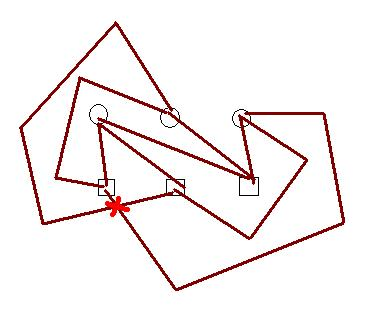
\includegraphics{bells.jpg}

Попробуйте вначале решить задачу самостоятельно, а потом читайте дальше.

{\bfseries Определение.} Граф, который возможно изобразить на плоскости без пересечения ребер, называется {\slshape планарным}.

Очевидно, что это ровно то, что нам требуется: надо проверить, является ли граф для домиков и колодцев планарным. Этот граф имеет специальное обозначение $K_{3, 3}$ и в простейшем виде, если не заморачиваться о пересечениях, может быть изображен так:

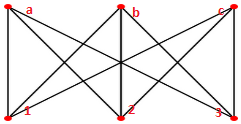
\includegraphics{k331.png}

Можно ли его нарисовать без пересечения линий? Для начала запишем его ребра в виде множества: $E = \{a1, a2, a3, b1, b2, b3, c1, c2, c3, \ldots\}$ Для удобства мы не стали перечислять симметричные отношения (понятно, что если $a1\in E$, то и $1a \in E$ и лишний раз упоминать это скучно) и ребра $(v, w)$ кратко записывали как $vw$.

{\bfseries Определение.} Граф $G' = (V', E')$ называется {\slshape подграфом} графа $G = (V, E)$, если $V' \subset V$ и $E' \subset E$.

Рассмотрим такое подмножество ребер: $C = \{a1, 1b, b2, 2c, c3, 3a\}$. Эти ребра образуют такой подграф:

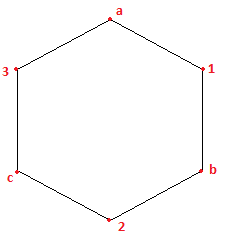
\includegraphics{cycle.png}

Подобные последовательности имеют специальные названия. Просто упомянем их для порядку:

{\bfseries Определение.} Последовательность чередующихся вершин и ребер, в которой каждое ребро стоит между различными вершинами, которым оно инцидентно, называется {\slshape путем}.

В нашем случае путь записывается как последовательность $a, a1, 1, 1b, b, b2, 2, 2c, c, c3, 3, 3a, a$.

{\bfseries Определение.} Если в пути нет повторяющихся ребер, то он называется {\slshape цепью}.

{\bfseries Определение.} Если первая и последняя вершины цепи совпадают, то такой путь называется {\slshape замкнутой цепью}, либо {\slshape циклом}. Если не совпадают, то цепь {\slshape незамкнута}.

Приведенный нами подграф $C$ очевидно является циклом и иллюстрация дает понять откуда берется такое называние. И хочешь не хочешь, но как этот цикл не рисуй он всегда либо будет иметь самопересечения, либо будет разбивать плоскость на две части: внутреннюю и внешнюю, и в этом смысле наш цикл имеет простейший вид какой только возможно (По хорошему это тоже надо строго доказывать да и вообще определять что значит «разбивает плоскость», но мы это сделаем намного позже, когда будем говорить о геометрии, а пока что просто доверимся интуиции).

Множество рёбер нашего первоначального графа $E = C \cup \{a2, b3, c1\}$ и нам необходимо дорисовать к подграфу $C$ три ребра, чтобы получить $E$. Здесь можно просто рассмотреть все возможные варианты. Если нарисовать $a2$ внутри цикла, то $b3$ и $c 1$ должны быть снаружи цикла, иначе они будут пересекать ребро $a2$. Но оба ребра $b3$ и $c 1$ тоже не могут быть одновременно снаружи, так как в этом случае они так же будут пересекаться. Значит, $a2$ не может быть нарисован внутри цикла так, чтобы граф $K_{3, 3}$ не имел пересечений. Однако если нарисовать $a2$ снаружи цикла, то так же можно увидеть, что $b3$ и $c 1$ неминуемо пересекутся внутри цикла. Таким образом мы перебрали все возможные варианты и убедились:

{\bfseries Лемма.} Граф $K_{3, 3}$ не является планарным.

Это ровно то что требовалось выяснить в условиях задачи.

Термин «лемма» обычно (но не всегда) используется для обозначения промежуточных результатов, которые будут задействованы далее в каких-то более сильных утверждениях. Самостоятельно предлагаю доказать вам еще следующую лемму:

{\bfseries Лемма.} Граф $K_5$ имеющий вершины $\{a, b, c, d, e\}$, каждая пара которых инцидентна, не планарен.

В простом виде этот граф выглядит так:

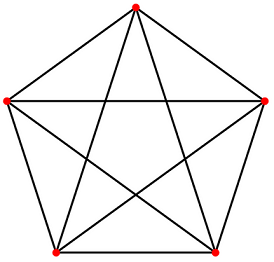
\includegraphics{k5.png}

Его не планарность доказывается так же, как и в случае с графом $K_{3, 3}$.

Из двух лемм, сформулированных выше, можно получить такую теорему:

{\bfseries Теорема.} Граф, который содержит в качестве подграфов $K_{3, 3}$ или $K_5$ не планарен.

Оказывается, что наличие подграфов, которые структурно схожи с $K_{3, 3}$ или $K_5$ является и необходимым условием. «Структурно схожи» можно выразить строго следующими терминами (в следующих определениях я опять не упоминаю симметричных отношений для краткости):

{\bfseries Определение.} Пусть дан граф $G=(V, E)$ и $(a, b) \in E$. Тогда {\slshape разбиением} графа $G$ по дуге $(a, b)$ называется граф $G' = (V\cup\{x\}, E\cup\{(a, x), (x, b)\}\setminus\{(a, b)\})$.

{\bfseries Определение.} Графы $A$ и $B$ называются {\slshape гомеоморфными}, если существует граф, такой что оба графа $A$ и $B$ получаются из него некоторыми разбиениеями дуг.

{\bfseries Теорема Куратовского.} Граф является планарным тогда и только тогда, когда он не содержит подграф, гомеоморфный $K_{3, 3}$ или $K_5$.

Разбиение графа — это вставка вершины посреди какого-то ребра. Эта операция, очевидно, не влияет на возможность нарисовать граф планарно: подразбиение это просто выделение точки на линии. Например, мы на каждой тропине от колодца к домику могли бы поставить опорный пункт полиции. Понятно, что граф уже не был бы равен $K_{3, 3}$, но в целом выглядел бы он точно так же.

Доказывать теорему Куратовского мы не будем, потому что я не знаю как ее доказывать, да и не особо она нужна по большому счету (в рамках этого курса точно не пригодится). Я когда сам в свое время начинал читать доказательство, мне оно показалось скучным и длинным, и я бросил это занятие. Если хотите, можете найти доказательство в Интернете. Однако зато теперь, если вам кто-то предложит решить головоломку с колодцами и домиками, вы можете с умным видом заявить: «Эта задача не имеет решения по теореме Куратовского», — и все сразу подумают, что вы умный. Я подобным образом пытался даже когда-то соблазнять девчонок (я правда рассказывал им о теореме Гёделя о неполноте), но это ни к чему так и не привело. Как был одинокий хрен так и остался.

Шутки шутками, но я бы хотел обратить внимание на то зачем я вообще завел речь об этой задаче. По ходу изложения мы активно использовали терминологию теории множеств. Могли бы мы обойтись без нее? Вообще говоря да. В теории множеств у нас не было никаких особых теорем, которыми бы мы тут воспользовались, и мы вполне могли провести все те же рассуждения и не обращаясь к множествам и определению графа. Какие-то понятия нам все равно пришлось бы вводить, но это не сложно. Тем не менее теория множеств дала нам язык, на котором мы смогли это все строго сформулировать, а заодно дала нам какие-то общие идеи, хоть и очень простые, как вообще можно поступать с этими графами.

Следующая задача тоже может быть решена без теории множеств и теории графов, но однако если к задаче с колодцами еще можно было как-то подступиться без множеств, то тут это уже вряд ли получится, хотя, опять же, напрямую свойства множеств никак не используются (замечу, что теоретический материал тут будет довольно сложный, так что при первом прочтении можно его и пропустить).

{\bfseries Задача.} В некоторой компании работает некоторое количество менеджеров. Директор вынудил их играть в странную игру. Каждому из менеджеров он надевает либо черную, либо белую шапку на голову. Менеджеры не знают цвета своей шапки, но видят цвет шапок других менеджеров. В какой-то момент в комнате звенит звонок и менеджеры должны одновременно по звонку назвать цвет собственной шапки (то есть менеджер называет цвет шапки, которую он не видит). Называть цвет должны не обязательно все — кто-то может и промолчать, но те кто называют цвет, должны делать это одновременно. Если хоть один менеджер ошибется, то увольняют всех.  Если все промолчат, то тоже всех увольняют. Если же все, кто все же осмелится назвать цвет своей шапки, назовут его правильно, то все получают повышение. У них всего одна попытка и никак переговариваться/перемигиваться они не могут, называть цвета последовательно они тоже не могут — лишь одновременно и с первой попытки. Вопрос: как быть менеджерам?

Здесь надо отметить, что конечно же гарантированного способа избежать увольнения у менеджеров нет. Каждый менеджер и вправду не может знать своего цвета шапки, поэтому всегда есть шанс, что менеджер, называющий свой цвет, ошибется. Однако поступая мудро, шанс ошибки можно минимизировать. Попробуйте вначале решить задачу самостоятельно, а затем читайте дальше. Для произвольного количества менеджеров задача действительно сложна, но для трех менеджеров, довольно легко придумать простое и интуитивно-понятное решение. (Его я сформулирую в самом конце). Пока же обратимся опять к теории множеств и графов и посмотрим что можно сделать с этой задачей.

{\bfseries Определение.} Пусть даны графы $G_0 = (V_0, E_0)$ и $G_1 = (V_1, E_1)$. Их {\slshape декартовым произведением} называется граф $G_0 \square G_1 = (V, E)$, такой что $V = V_0 \times V_1$ и $((a, b), (v, w)) \in E$ тогда и только тогда, когда либо $a=v$ и $(b, w) \in E_1$, либо $b=w$ и $(a, v) \in E_0$.

В новом графе вершины записываются как упорядоченные пары из $V_0 \times V_1$ и  соответственно ребра этого графа являются упорядоченными парами упорядоченных пар, что формально можно записать так:

$E \subset (V_0\times V_1)\times(V_0\times V_1) \\ E = \{((a, b), (v, w))|(a=v \wedge (b, w)\in E_1)\vee(b=w \wedge (a, v)\in E_0)\}$

Выглядит чудовищно, но если вдуматься, то это вполне логичное и естественное определение для ребер, если задавать его на произведении $V_0 \times V_1$. Тут вероятно помогут примеры.

Обозначим как $K_2$ простенький граф, состоящий из двух вершин, соединенных ребром ($V = \{0, 1\}$, $E = \{(0, 1), (1, 0)\}$).

Тогда можно увидеть, что в соответствии с определением $K_2$:

\begin{picture}(20,75)
\put(10,0){0}
\put(12,10){\line(0,1){50}}
\put(10,64){1}
\end{picture}

Его декартово произведение самого с собой $K_2 \square K_2$:

\begin{picture}(20,75)
\put(5,0){(0,0)}
\put(5,66){(1,0)}
\put(55,0){(0,1)}
\put(55,66){(1,1)}
\put(12,11){\line(0,1){50}}
\put(12,11){\line(1,0){50}}
\put(62,61){\line(0,-1){50}}
\put(62,61){\line(-1,0){50}}
\end{picture}

Умножим это еще раз на него же ($K_2 \square K_2 \square K_2$, так как вершин много, я на этот раз указываю лишь некоторые из них):

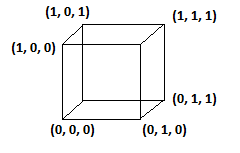
\includegraphics{k23.png}

И еще раз ($K_2 \square K_2 \square K_2 \square K_2$):

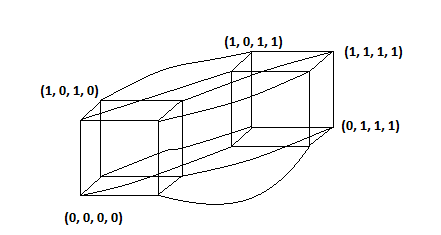
\includegraphics{k24.png}

Тут так и напрашиваются геометрические ассоциации, и это в общем-то неспроста. Действительно, на рисунках по сути изображены отрезок, квадрат, куб и, как мы позже выясним, четырехмерный куб (в свою очередь так же выяснится, что квадрат — это двумерный куб, а отрезок — одномерный куб). По сути каждый раз умножая наш граф на $K_2$, мы вводим еще одно измерение, в котором мы копируем наш куб, и эти два куба склеиваем по вершинам. Четырехмерный куб (то есть его граф), приведенный выше, можно нарисовать в четырехмерном пространстве без пересечения ребер графа. Вообразить себе такое пространство и такой куб оказывается довольно сложно, но представление в виде графов дает об этих кубах (и вообще многомерных объектах) довольно много информации. Например, из рисунка выше мы видим сколько всего у четырехмерного куба будет вершин и ребер, какие вершины какими ребрами соединены, сколько из каждой вершины исходит ребер и так далее. Это согласитесь уже не мало.

Развивая идею можно заметить, что декартово произведение графов ассоциативно и с точностью до переименования вершин коммутативно (и вообще тут можно построить целую арифметику графов при желании, так же как мы поступали с логическими операциями и операциями на множествах). Отсюда в силу ассоциативности сразу следует, что декартово произведение многомерных кубов — тоже является многомерным кубом, и можно сразу понять размерность такого куба.

Топологические приложения изложенного материала идут еще дальше. Есть довольно общий приём триангуляции — разукрашивание поверхностей прилегающими друг к другу треугольниками. Каждая триангуляция является графом. Поверхности называются гомеофорфными, если, представляя, будто они сделаны из резины, можно одну поверхность как-то продеформировать (растянуть-перекрутить без разрывов и склеиваний) в другую поверхность. Это довольно близко к понятию гомеоморфности графов. Позже мы докажем в нашем курсе, что если две поверхности возможно триангулировать гомеоморфными графами, то эти две поверхности сами гомеофорфны, а конструкции, подобные декартову произведению, позволяют выяснить это сравнительно простым путем. Более того, гомеоморфность — это отношение эквиваленции, и таким образом все поверхности распадаются на классы топологически-эквивалентных поверхностей. Дальше на эти классы эквивалентности можно завязать всяческую алгебру и углубляться дальше в абстрактные конструкции сколько вздумается.

Эти рассуждения конечно очень абстрактны и не строги, и пока не очень понятно как именно все это описывается и как с этим работать. Я это рассказал только в обзорных целях для того, чтобы показать куда это все вообще может развиваться, поскольку читатели жалуются, что курс слишком теоретический и не практичен.

{\bfseries Упражнение.} Пусть $P$ — незамкнутая цепь. Постройте (и нарисуйте) граф $P\square K_2$ (такой граф называется лестницей).

{\bfseries Упражнение.} Пусть опять $P$ — незамкнутая цепь. Постройте (и нарисуйте) граф $P\square P$ (такой граф называется сетью).

Следующие упражнения можно решать только при наличии каких-то геометрических образов в голове. Я их никак не объяснял, поэтому материала курса пока явно не хватит для решения, однако вы можете их хотя бы попробовать. Если вы ничего не понимаете, то это не страшно (и даже справедливо), смело пропускайте их — далее в курсе это всё будет рассмотрено более подробно и формально, и тогда к ним можно будет вернуться.

{\bfseries Упражнение.} Докажите, что куб, пирамида и сфера гомеоморфны (их можно триангулировать одним и тем же графом; вершины графа не обязательно могут совпадать с геометрическими вершинами трехмерного объекта — важна лишь возможность его нарисовать).

{\bfseries Упражнение.} Докажите, что если $C$ — это цикл, то $C\square P$ — это цилиндр, и что цилиндр гомеоморфен сфере.

{\bfseries Упражнение.} Докажите, что $C\square C$ — это тор (выглядит как бублик) и он не гомеоморфен сфере.

В общем случае, если нам даны графы $A$ и $B$, то их произведение $A\square B$ строится, как теперь должно быть понятно, следующим образом: каждая отдельная вершина графа $B$ заменяется на точную копию графа $A$, а ребра графа $B$ соответственно заменяются на ребра, соединяющие все соответствующие вершины копий графа $A$.

Но вернемся к нашим менеджерам. Какое они имеют отношение ко всей этой многомерной геометрии? А вот какое.

Каждого менеджера можно условно считать графом $K_2$. Одна вершина этого графа символизирует белую шапку на нём, другая черную, а ребро, их соединяющее — тот факт, что для него эти цвета неразличимы (он не видит какая шапка на нем надета). Тогда несколько менеджеров можно интерпретировать как многомерный куб $K_2 \square K_2 \square \ldots \square K_2$, у которого каждая вершина соответствует некоторому набору шапок на менеджерах. В момент, когда на менеджеров надевают шапки, фактически совершается выбор одной вершины куба. Но никакой отдельный менеджер не знает что это за вершина, так как он не знает цвета собственной шапки — он знает лишь то, что он «находится» в одной вершине куба из двух, то есть его знание может быть охарактеризовано ребром куба.

Пусть, например менеджеров трое, и всем надели белые шапки, что мы будем записывать как $(0, 0, 0)$. Первый менеджер не знает какая на нем надета шапка, и для него выбор стоит между $(0, 0, 0)$ и $(1, 0, 0)$. Для второго между $(0, 0, 0)$ и $(0, 1, 0)$. Для третьего $(0, 0, 0)$ и $(0, 0, 1)$. Это и есть ребра, которые исходят из вершины, характеризующей расстановку шапок.

После того, как менеджеры увидели шапки друг друга, им надо принять решение какой цвет назвать и называть ли его вообще. Поведение менеджеров таким образом можно описать ориентированным графом с теми же вершинами, но где каждое ребро либо удалено, либо заменено на дугу (ребро, направленное в одну сторону). Продолжая прошлый пример, если первый менеджер выберет сказать, что у него белая шапка, это будет представлено дугой $(1,0,0)\to (0, 0, 0)$, если предпочтет сказать, что шапка черная, то это будет дуга $(0, 0, 0)\to (1, 0,0)$. Если предпочтет промолчать, то вершины $(0, 0, 0)$ и $(1, 0, 0)$ вообще не будут инцидентны.

Попытаемся понять, как нам надо выбрать этот орграф таким образом, чтобы менеджеры в большинстве случаев справлялись с задачей. Если у нас в некоторую вершину идет хоть одна дуга, то это значит, что если расстановка шапок будет соответствовать этой вершине, то кто-то из менеджеров назовет цвет своей шапки. Если из какой-то вершины исходит какая-то дуга в другую вершину, то это значит, что при расстаноке шапок для этой вершины менеджер, соответствующей этой дуге, ошибется, и все проиграют. Если какая-то вершина не будет инцидентна никакой другой вершине, то это значит, что при соответствующем расположении шапок, все промолчат, и менеджеры снова проиграют.

Наша задача сводится к такому заданию ориентированного графа, чтобы количество проигрышных вершин (таких, из которых исходят дуги), было как можно меньше, и как можно больше вершин, в которые идет хотя бы по одной стрелке, но для которых нет исходящих стрелок. Такую оптимальную стратегию для трех менеджеров можно выразить следующим рисунком:

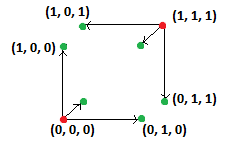
\includegraphics{sol3.png}

Здесь фактически говорится, что если некий менеджер видит, что шапки двух других менеджеров имеют одинаковый цвет, то ему надо назвать цвет противоположный. Это действительно очень простая стратегия: вероятность того, что всем оденут шапку одного цвета меньше, чем вероятность того, что цвета будут все же разными. Поэтому можно предполагать, что существуют все же разноцветные шапки, и поэтому если ты видишь, что у двух менеджеров одинаковые шапки, то на тебе самом с большой степенью вероятности шапка имеет противоположный цвет. До этого решения конечно можно было бы догадаться и без многомерных кубов.

А вот решение для четырех менеджеров:

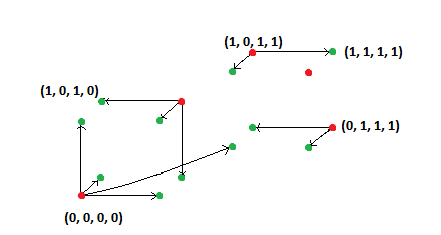
\includegraphics{sol4.png}

Эту стратегию уже так просто не сформулируешь. Если все четверо видят только белые шапки, то надо называть черный цвет. Во всех остальных ситуациях четвертый менеджер вообще молчит, говорят оставшиеся. Если на всех кроме четвертого черные шапки, то все кроме четвертого называют белый цвет. Если на четвертом менеджере черная шапка, то первый менеджер должен молчать. Если второй видит на третьем и четвертом черные шапки, то он должен называть цвет, который видит на первом менеджере. Третий же менеджер должен называть цвет второго менеджера, если он не совпадает с цветом первого. В остальных случаях менеджеры молчат. (Вероятно я где-то ошибся, потому что глядя на этот график можно глаза сломать и я не уверен, что корректно его прочитал; но идея думаю понятна). Решение с трудом можно назвать изящным, но как видно из нашего графа, в большинстве случаев менеджеры все же будут выигрывать. Поэтому это пусть и не красивое (и даже уродливое), но все равно решение. Согласитесь, что если бы это был вопрос жизни и смерти, то оно бы вас устроило.

Если менеджеров больше, то задача решается аналогично, хотя графы будут еще больше по размеру и перебирать придется еще больше вариантов. С этим может справиться компьютер, хотя задача все равно сложная. Какого-то универсального и простого решения к этой задаче видимо не существует, но тем не менее с помощью графов мы смогли получить хоть что-то. Без подобных абстракций и строгой формализвации, задача не решалась бы вообще никак.

Еще хуже была бы ситуация, если бы цветов шапок было бы не два, а больше. Тогда помогло бы следующее понятие:

{\bfseries Определение.} {\slshape Гиперграфом} называется пара $(V, E)$, где $E\subset 2^V$.

Фактически это граф, в котором ребра соединяют сразу множество вершин.

Любой гиперграф может быть представлен с помощью обычного графа. Для этого надо рассмотреть граф, множество вершин которого разбито на два подмножества — одно подмножество вершин соответствует вершинам гиперграфа ($V_0$), а второе ребрам гиперграфа ($V_1$). Множество ребер, инцидентных одной и той же вершине из $V_1$ соответствует грани гиперграфа.

Используя гиперграфы можно решать задачу менеджеров и с произвольным количеством цветов шапок. Задача однако в этом случае становится менее интересной, так как вероятность выигрыша менеджеров резко падает.

Гиперграф — не единственное возможное обобщения понятия граф. Гораздо чаще применяется следующее определение:

{\bfseries Определение.} {\slshape Абстрактным симплициальным комплексом} на множестве $S$ называется множество $\Delta\subset 2^S$, такое, что если $x\in \Delta$, то для любого $y\subset x$ так же $y\in\Delta$. Элементы множества $\Delta$ называются {\slshape абстрактными симплексами}.

Абстрактные симплициальные комплексы удобно строить последовательно: вначале выбирается множество вершин $S$ (так называемые нульмерные симплексы). Затем выбираются обычные ребра графа, соединяющие вершины из $S$ (одномерные симплексы). Затем из различных объединений этих ребер и вершин выбираются трехмерные симплексы, которые можно рассматривать как сплошные пленки, которыми заклеиваются ребра графа. Объединяя эти пленки можно выбрать трехмерные симплексы, затем четырехмерные и так далее. Здесь правда надо следить за тем, чтобы «наклеивая пленки» мы не нарушали условий определения комплекса. Например, если есть грани $\{a, b\}$ и $\{b, c\}$, но нет грани $\{a, c\}$, то наклеить пленку $\{a, b, c\}$ мы не имеем права, поскольку по определению для ее наклеивания требуется так же наличие грани $\{a, c\}$, что неплохо соответствует геометрической интуиции.

Такие конструкции используются опять же в многомерной топологии и с помощью них можно выяснять подробности устройства многомерных объектов. В этом курсе все это будет значительно позже, пока что я привел эти определения лишь для того, чтобы показать каким образом самые базовые понятия теории множеств могут быть полезны простому человеку и как она позволяет простым способом обобщать привычные в общем-то понятия. Написанное в этом параграфе можно смело забыть до поры, это все у нас будет значительно позже.
